% Generated from step0194 own-clock reanalysis by step0195.
% Actual error classes at left; conditional constant-work models at right.
\begin{minipage}[t]{0.48\textwidth}
\centering
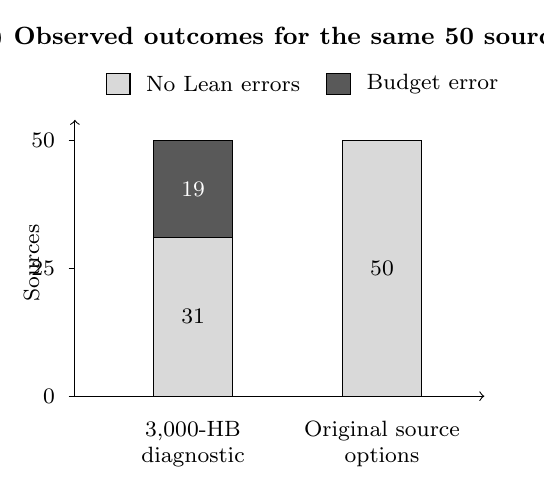
\begin{tikzpicture}[x=1cm,y=0.065cm,font=\footnotesize]
\path[use as bounding box] (-0.6,-14) rectangle (5.6,72);
\node[font=\small\bfseries] at (2.5,70) {(a) Observed outcomes for the same 50 sources};
\draw[->] (0,0) -- (5.2,0);
\draw[->] (0,0) -- (0,54);
\foreach \v in {0,25,50} {
 \draw (-0.08,\v) -- (0,\v);
 \node[anchor=east] at (-0.13,\v) {\v};
}
\node[rotate=90] at (-0.55,26) {Sources};
\draw[fill=black!15] (1,0) rectangle (2,31);
\draw[fill=black!65] (1,31) rectangle (2,50);
\draw[fill=black!15] (3.4,0) rectangle (4.4,50);
\node at (1.5,15.5) {31};
\node[text=white] at (1.5,40.5) {19};
\node at (3.9,25) {50};
\node[align=center,anchor=north] at (1.5,-3) {3,000-HB\\diagnostic};
\node[align=center,anchor=north] at (3.9,-3) {Original source\\options};
\draw[fill=black!15] (0.4,59) rectangle (0.7,63);
\node[anchor=west] at (0.78,61) {No Lean errors};
\draw[fill=black!65] (3.2,59) rectangle (3.5,63);
\node[anchor=west] at (3.58,61) {Budget error};
\end{tikzpicture}
\end{minipage}\hfill
\begin{minipage}[t]{0.48\textwidth}
\centering
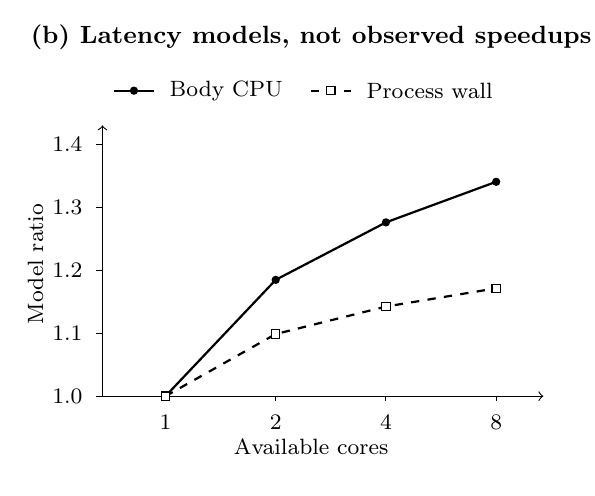
\begin{tikzpicture}[x=1cm,y=8cm,font=\footnotesize]
\path[use as bounding box] (-0.95,-0.114) rectangle (5.9,0.585);
\node[font=\small\bfseries] at (2.65,0.57) {(b) Latency models, not observed speedups};
\draw[->] (0,0) -- (5.6,0);
\draw[->] (0,0) -- (0,0.43);
\foreach \v/\lab in {0/1.0,0.1/1.1,0.2/1.2,0.3/1.3,0.4/1.4} {
 \draw (-0.08,\v) -- (0,\v);
 \node[anchor=east] at (-0.13,\v) {\lab};
}
\node[rotate=90] at (-0.85,0.21) {Model ratio};
\foreach \x/\lab in {0.8/1,2.2/2,3.6/4,5.0/8} {
 \draw (\x,0) -- (\x,-0.008);
 \node[anchor=north] at (\x,-0.015) {\lab};
}
\node at (2.65,-0.080) {Available cores};
\draw[thick] plot coordinates {(0.800,0.000000000) (2.200,0.184675298) (3.600,0.275923176) (5.000,0.340366751)};
\draw[thick,dashed] plot coordinates {(0.800,0.000000000) (2.200,0.098627390) (3.600,0.142253311) (5.000,0.171287111)};
\fill (0.800,0.000000000) circle[radius=1.5pt];
\fill (2.200,0.184675298) circle[radius=1.5pt];
\fill (3.600,0.275923176) circle[radius=1.5pt];
\fill (5.000,0.340366751) circle[radius=1.5pt];
\draw[fill=white] (0.800,0.000000000) ++(-1.5pt,-1.5pt) rectangle ++(3pt,3pt);
\draw[fill=white] (2.200,0.098627390) ++(-1.5pt,-1.5pt) rectangle ++(3pt,3pt);
\draw[fill=white] (3.600,0.142253311) ++(-1.5pt,-1.5pt) rectangle ++(3pt,3pt);
\draw[fill=white] (5.000,0.171287111) ++(-1.5pt,-1.5pt) rectangle ++(3pt,3pt);
\draw[thick] (0.15,0.485) -- (0.65,0.485);
\fill (0.4,0.485) circle[radius=1.5pt];
\node[anchor=west] at (0.73,0.485) {Body CPU};
\draw[thick,dashed] (2.65,0.485) -- (3.15,0.485);
\draw[fill=white] (2.9,0.485) ++(-1.5pt,-1.5pt) rectangle ++(3pt,3pt);
\node[anchor=west] at (3.23,0.485) {Process wall};
\end{tikzpicture}
\end{minipage}
